\chapter{Data Driven Classification of P Cygni and Inverse P Cygni Spectra}

\section{A Framework for Classification}

It is clear from the prior chapter that a classification approach to P Cygni and inverse P Cygni spectra must follow a morphology based scheme. While morphological classification based on naked eye observations of spectra has been used in the past, this approach cannot scale with the volume of data present in million star sky surveys and certainly cannot scale effectively on DR3. In terms of automated methods that can scale more effectively, approaches such as t-SNE and autoencoders \cite{traven2017galah,vcotar2021galah} have been successful in detecting H$\alpha$ emission spectra. While the former was not able to reliably identify a broader sample of these candidate spectra, the latter was able to identify several thousand potential H$\alpha$ spectra in DR3 using an anomaly detection approach (autoencoders). These recent methods, and notably latter have shown the greatest success in identifying H$\alpha$ candidates in DR3. However they fall short in the automated identification of P Cygni and inverse P Cygni spectra in DR3.

Given that DR3 does not have suitable labeled samples of P Cygni and inverse P Cygni spectra, a supervised learning approach to classification is not suitable. This narrows the field of possible technical and scientific approaches to the unsupervised classification domain \cite{hastie2009elements}. A classification approach that is sensitive to the meaningful morphological differences between P Cygni and inverse P Cygni also remains an important requirement. Feature engineering tasks that need to be performed to prepare the raw data must take into account the understanding that P Cygni spectra exhibit a red shifted emission peak while the inverse P Cygni spectra exhibit a blue shifted peak. Finally, given that the feature space is $\approx$ \num[round-precision=2,round-mode=figures, scientific-notation=true]{2928752091}, the classification approach must be able to grapple with this dimensionality and overcome the "curse of dimensionality".

\section{Time Series Clustering}

A full treatment of unsupervised clustering and classification methods is beyond the scope of this work, however this section will briefly introduce time series clustering, more specifically unsupervised time series clustering. It was noted in a prior chapter that DR3 spectra and indeed all spectra can be modeled as "time series". While an individual spectrum does not contain a time axis, the monotonically increasing wavelength grid serves as the analogue of the time axis in the context of traditional numerical computing methods. These machine learning methods have been more generally developed in the domain of time series analysis \cite{nielsen2019practical} and can be suitably adapted to stellar spectra. With clustering, we do not rely on labelled data, but rather develop a suitable method to cluster similar spectra into groups. Similar in this context being morphologically similar spectra such as P Cygni and inverse P Cygni.

\subsection{Dynamic Time Warping}

Dynamic time warping (DTW) is a time series analysis algorithm that can measure similarity between two temporal sequences. The similarity can then be used to cluster similar spectra into meaningful groups. These clusters can then be used to classify spectra into distinct classes. DTW is suitable for clustering problems where the morphology of the signal plays a salient role \cite{nielsen2019practical}. The name of the algorithm itself is inspired by the methodology where two signals are warped to align them on the temporal domain. For stellar spectra, this warping takes place in the wavelength domain. 

\begin{figure}[h]
\centering
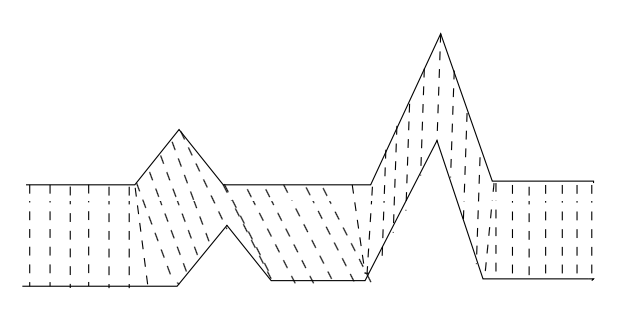
\includegraphics[scale=0.90]{figures/Dynamic_time_warping.png}
\caption{Each point on the wavelength grid is mapped to a point on the opposite spectrum, but there is no requirement that the mapping is one to one. Reproduced from Nielsen \cite{nielsen2019practical}}
\end{figure}

As indicated in the figure above, expansion or contraction of the wavelength axis to find the best alignment ensures that the shape of the spectra (the morphology) play a dominant role in determining similarity. This algorithm is often described as being akin to comparing the visual "shape" of the spectra, rather than focusing on the sequence of how these shapes are formed on the wavelength axis. The implications of this will be discussed in detail in this chapter. The algorithm follows a number of constraints which are,

\begin{enumerate}
    \item Every point on the spectrum must be matched with at least one point of the other spectrum
    \item The first and last indices of each spectrum must be matched with their counterparts in the other spectrum
    \item The mapping must be such that the wavelength is increasing rather than decreasing i.e. do not match a point on on spectrum to a point on the other spectrum that has "passed"
\end{enumerate}

Points 2 and 3 above do not have a significant impact on the DR3 dataset being used in this research as they are sampled to the same wavelength and thus are of equal length. There are many possible ways to align two spectra while adhering to these constraints. The algorithm chooses the match that minimises the distance between the spectra. This distance is a cost function and is measured as the sum of the absolute differences between matched points. The absolute difference in this context is the difference between the points values (wavelength values). Note that it is this distance measure that this research relies on to serve as the basis for clustering similar spectra into groups or classes.

The Pythonic representation of this algorithm is as follows,

\begin{lstlisting}[language=Python]
# Primary function
def distDTW(lambda1, lambda2):
     DTW={}
     for i in range(len(lambda1)):
         DTW[(i, -1)] = np.inf
     for i in range(len(lambda2)):
         DTW[(-1, i)] = np.inf
     DTW[(-1, -1)] = 0
 
# Calculate the optimum i.e. where distance is minimum
     for i in range(len(lambda1)):
         for j in range(len(lambda2)):
             dist = (lambda1[i] - lambda2[j])**2
             DTW[(i, j)] = dist + min(DTW[(i-1, j)],
                                      DTW[(i, j-1)], 
                                      DTW[(i-1, j-1)])
 
 # Return the associated distance between two spectra
     return sqrt(DTW[len(lambda1)-1, len(lambda2)-1])
\end{lstlisting}

Despite the effectiveness of this algorithm, the computational complexity is of order $O(N^2)$. As this presents a significant computational cost and overhead, this research relies on a linear time complexity i.e. $O(N)$ implementation of DTW called \texttt{FastDTW} to compute the optimum distance between spectra and thus the similairty \cite{salvador2007toward}. \texttt{FastDTW} is a linear approximation to the DTW method above and a full discussion is beyond the scope of this thesis. 

In addition to computational complexity, an important consideration when running DTW is available memory. All spectral data must be loaded into memory (RAM) when computing DTW distances. In the case of DR3, this implies holding $\sim$ \num[round-precision=2,round-mode=figures, scientific-notation=true]{2928752091} features in memory. The computational hardware available for this project had a memory capacity of $\sim$ 300 GB. DTW required a memory capacity of at least 1TB for the $\sim$ \num[round-precision=2,round-mode=figures, scientific-notation=true]{2928752091} features. This is a significant amount of data to hold in memory. 

This research presents two strategies to overcome these limitations and reduce computational and memory overheads.

\begin{enumerate}
    \item Reduce the number of features - As explained in a prior chapter, this research will pre-select only the region around H$\alpha$. DTW will be run on this region only.
    \item Reduce the search space from the entire DR3 dataset to a subset which has a higher chance of yielding P Cygni and inverse P Cygni spectra - The existence of H$\alpha$ emission features is a precursor to the existence of P Cygni and inverse P Cygni features in a spectrum. Thus this research uses a DR3 H$\alpha$ emission candidate dataset from Čotar et al.\cite{vcotar2021galah}. This subset with $\sim$ 10,000 candidates includes data from both DR3 and other related surveys. Presumably, this dataset only contains H$\alpha$ emission candidates and not typical spectra.
\end{enumerate}

Taken together, these strategies reduce the feature space from $\sim$ \num[round-precision=2,round-mode=figures, scientific-notation=true]{2928752091} to a more manageable feature space of size $\sim$ \num[round-precision=2,round-mode=figures, scientific-notation=true]{45228200}.

\subsection{Agglomerative Hierarchical Clustering}

Given a similarity measure, or in the case of DTW, pairwise distance measurements, hierarchical clustering can be used to group similar spectra into clusters. Once a similarity measure (or a dissimilarity measure) has been specified, they produce a hierarchical representation in which clusters at each level of the hierarchy are created by merging clusters at the next lower level. At the lowest level, each cluster contains a single observation. At the highest level, there exists a single cluster that contains all of the data \cite{hastie2009elements}.There are two basic paradigms to traverse these levels or "tree", aggolomerative (bottom-up) and divisive (top-down). 

With agglomerative clustering, each spectrum will form a singleton cluster. At each step, the most similar spectra will be merged into a single cluster, producing one less cluster at the next higher level. The similarity between two spectra is defined as the DTW distance between them. Lower distances imply a greater similarity while greater distances indicate a dissimilarity. 

Based on the similarity (and dissimilarity) between individual spectra, a cluster dissimilarity can also be defined. Consider two clusters in such a scheme called $A$ and $B$. The dissimilarity between the two clusters $d(A,B)$ is computed from the set of pairwise observation dissimilarities $d_{ij}$, where one member of the pair $i$ is in $A$ and the other $j$ is in $B$. The \emph{complete linkage dissimilarity} between the two clusters is set to be the dissimilarity of the furthest (most dissimilar) pair of spectra

\begin{equation}
    d(A,B) = \max_{\substack{i \in A \\ j \in B}} d_{ij}
\end{equation}

This is also known as the farthest neighbour technique. Other dissimilarity measures such as \emph{single linkage dissimilarity} or nearest neighbour dissimilarity can be defined as

\begin{equation}
    d(A,B) = \min_{\substack{i \in A \\ j \in B}} d_{ij}
\end{equation}

Hierarchical clusters can be visualised using a dendogram. A dendogram is a binary tree that represents the recursive agglomeration (or division). The height of the tree (or a branch) is proportional to the inter-group dissimilarity defined above. 

\begin{figure}[h]
\centering
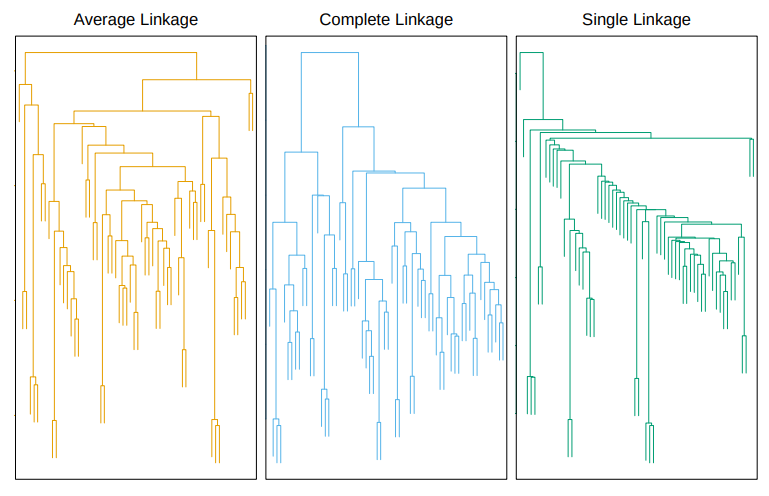
\includegraphics[scale=0.60]{figures/complete linkage.png}
\caption{Dendograms for the same dataset using different measures. Note the longer branch lengths of the complete linked tree that selects for maximum dissimilarity. Reproduced from Hastie et al.\cite{hastie2009elements}}
\end{figure}

This research uses the complete linkage dissimilarity to cluster spectral groups. The justification for using this measure over the single linkage dissimilarity is to force the separation of P Cygni and inverse P Cygni spectra into distinct groups by exploiting the maximum distance between two individual spectra that belong to these groups. Other distance measures such as group average clustering uses the average dissimilarity between the groups. This research does not consider this measure as it may be less accurate in separating P Cygni from inverse P Cygni. A full discussion of the advantages and disadvantages of each approach is beyond the scope of this thesis. This research also relies on the agglomerative paradigm as it is more robust and has been studied extensively in the literature while the divisive paradigm has not been studied extensively \cite{hastie2009elements}.

\subsection{Selecting the Number of Clusters}

Given that the framework proposed above is an entirely unsupervised machine learning approach, it is generally not required that the cluster size be specified in advance. In the absence of a predefined cluster size, the typical approach would require a plot of the dendogram where suitable cuts be made at a required level. However since the tree can theoretically be cut at any level and can have a maximum cluster size equal to the number of samples and a minimum cluster size equal to 1, as will be demonstrated below, a more meaningful and reliable cut can be made with the aide of astrophysical domain knowledge. In the absence of such knowledge this research would have to cut the dendogram at each level, the examine the clusters and subsequently decide on a suitable cluster size. Furthermore, given that the sample size is at least 10,000 spectra, visually inspecting a dendogram for this dataset can be challenging. This research proposes the use of prior art to determine a cluster size in advance, thus eliminating the requirement to visually inspect a complex dendogram of the order of thousands of branches. 

While this research is focused on P Cygni and inverse P Cygni spectra, it is clear that other morphologies of H$\alpha$ candidates have been found using manual methods. Reipurth et al. in particular proposed the existence of seven morphological groups which include P Cygni and inverse P Cygni as well as five other H$\alpha$ emission morphologies \cite{reipurth1996halpha}. In order to only extract P Cygni and inverse P Cygni clusters, if the cluster size is set only to two, there is a significant risk that other morphologies will be included in the P Cygni cluster and inverse P Cygni cluster thus leading to erroneously classified/labelled clusters. Thus based on the prior art, this research takes cluster sizes between seven and ten to be a suitable range. The number of samples this research will subject to automated clustering will be significantly higher than any previous prior art, especially the manual classification approaches detailed in prior chapters. The justification to use a higher number of clusters such as ten is to account for the possibility of additional morphological classes that may have been missed in the prior art during manual observation. 